\documentclass{article}

\usepackage{lipsum}
\usepackage{amsfonts}
\usepackage{amsmath}
\usepackage{amsthm}
\usepackage{graphicx}
\graphicspath{{figures/4_28_22/}}
\usepackage{epstopdf}
\ifpdf%
\DeclareGraphicsExtensions{.eps,.pdf,.png,.jpg}
\else
\DeclareGraphicsExtensions{.eps}
\fi
\usepackage{amsopn}
\DeclareMathOperator{\diag}{diag}
\usepackage{booktabs}
\usepackage{bbm}
\usepackage{bm}
\usepackage{caption}
\usepackage{subcaption}
\usepackage[utf8]{inputenc}
\usepackage[T1]{fontenc}
\usepackage[margin=1in]{geometry}
\usepackage{hyperref}
\usepackage{algorithm}
\usepackage{algpseudocode}
\usepackage{placeins}

\newcommand{\norm}[1]{\left\lVert#1\right\rVert}
\newcommand{\normtwo}[1]{\left\lVert#1\right\rVert_2}
\newcommand{\abs}[1]{\left\lvert#1\right\rvert}
\newcommand{\mat}[1]{\bm{{#1}}}
\renewcommand{\vec}[1]{\bm{{#1}}}
\newcommand{\lequiv}{\Leftrightarrow}
\newcommand{\bigO}[1]{\mathcal{O}\!\left(#1\right)}
\newcommand{\ceil}[1]{\left\lceil #1 \right\rceil}
\newcommand{\floor}[1]{\left\lfloor #1 \right\rfloor}
\newcommand{\sfrac}[2]{#1/#2}
\newcommand{\hquad}{\enskip}
\newcommand{\expected}[1]{\mathbb{E}\left[#1\right]}
\newcommand{\mspan}[1]{\text{span}\left( #1 \right)}
\newcommand{\prob}[1]{P\left(#1\right)}
\newcommand{\probt}[1]{P\left( \text{#1} \right)}
\newcommand{\condprob}[2]{P\left(#1 \:|\: #2\right)}
\newcommand{\condprobt}[2]{P\left(\text{#1} \:|\: \text{#2}\right)}
\newcommand{\bayes}[2]{\frac{\condprob{#2}{#1}\prob{#1}}{\prob{#2}}}
\newcommand{\bayesx}[3]{\frac{\condprob{#2}{#1}\prob{#1}}{\condprob{#2}{#1}\prob{#1} + \condprob{#2}{#3}\prob{#3}}}
\newcommand{\sech}{\text{sech}}
\newcommand*{\vertbar}{\rule[-1ex]{0.5pt}{2.5ex}}
\newcommand*{\horzbar}{\rule[.5ex]{2.5ex}{0.5pt}}
\newcommand{\vect}[2]{\underline{{#1}}_{{#2}}}
\newcommand{\basisp}[1]{\underline{{p}}_{{#1}}}
\newcommand{\basisq}[1]{\underline{{q}}_{{#1}}}
\newcommand{\coeff}[1]{\underline{{a}}_{{#1}}}
\newcommand{\bestfit}{\underline{\bar{x}}}
\newcommand{\grad}{\nabla}
\newcommand{\laplace}{\Delta}
\newcommand{\setbar}{\:\middle|\:}
\renewcommand{\div}{\grad \cdot}
\renewcommand{\Re}{\text{Re}}
\newcommand{\var}[1]{\texttt{{#1}}}

\begin{document}
%% \section{Background}

Learning aggregation for 3D anisotropic diffusion on a structured grid
\begin{equation}
  -\grad \cdot \left(\mat{D} \grad u\right) = 0,
\end{equation}
\begin{equation}
  \mat{D} := \mat{R}^T\begin{bmatrix}\varepsilon_x & & \\ & \varepsilon_y & \\ & & 1 \end{bmatrix}\mat{R},
\end{equation}
\begin{equation}
  \mat{R} := \begin{bmatrix} \cos \theta_z & -\sin \theta_z & 0 \\ \sin \theta_z & \cos \theta_z & 0 \\ 0 & 0 & 1\end{bmatrix} \begin{bmatrix}\cos \theta_y & 0 & \sin \theta_y \\ 0 & 1 & 0 \\ -\sin\theta_y & 0 & \cos\theta_y \end{bmatrix}.
\end{equation}

Two sets of:
\begin{itemize}
\item 500 training problems, and
\item 250 testing problems
\end{itemize}
were generated to train the ML method.  These problems randomly have the parameters $N_x=N_y=N_z=N \sim \mathcal{U}\left\{8, 14\right\}$; $\theta_z, \theta_y \sim \mathcal{U}\left(0, 2\pi\right)$; $\log_{10}\varepsilon_x, \log_{10}\varepsilon_y \sim \mathcal{U}\left(-4, 4\right)$.

Each problem was discretized in Firedrake \cite{Firedrake} using piecewise linear tetrahedral finite elements with homogeneous Dirichlet boundary conditions.  Afterwards, the degrees-of-freedom corresponding to Dirichlet boundary conditions were removed from the system.

The network for 3D problems is still training, so the following results are for the existing 2D isotropic/anisotropic diffusion network evaluated on these problems.

\begin{table}[h]
  \centering
  \begin{tabular}{c c c c}
    \textbf{Data Set} & \textbf{Random Conv.} & \textbf{Lloyd Conv.} & \textbf{ML Conv.} \\
    \hline
    Train & 0.7088 & 0.7145 & 0.7209 \\
    Test & 0.7166 & 0.7234 & 0.7288 \\
    \hline
  \end{tabular}
  \caption{Convergence of ML vs baseline, Lloyd methods on both data sets.}
  \label{tab:conv}
\end{table}

\begin{figure}[!hb]
  \centering
  \begin{subfigure}[t]{0.49\textwidth}
    \centering
    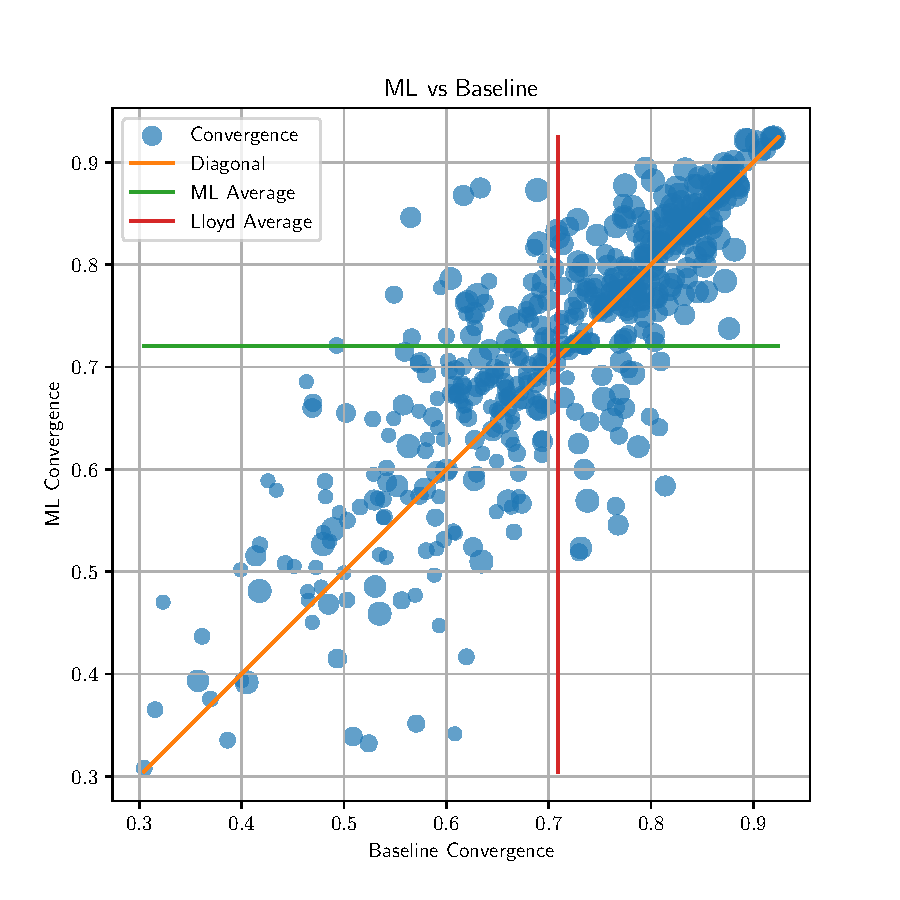
\includegraphics[width=\textwidth]{aniso3d_train_baseline_ml_convergence.pdf}
    \caption{Training convergence}
  \end{subfigure}
  \begin{subfigure}[t]{0.49\textwidth}
    \centering
    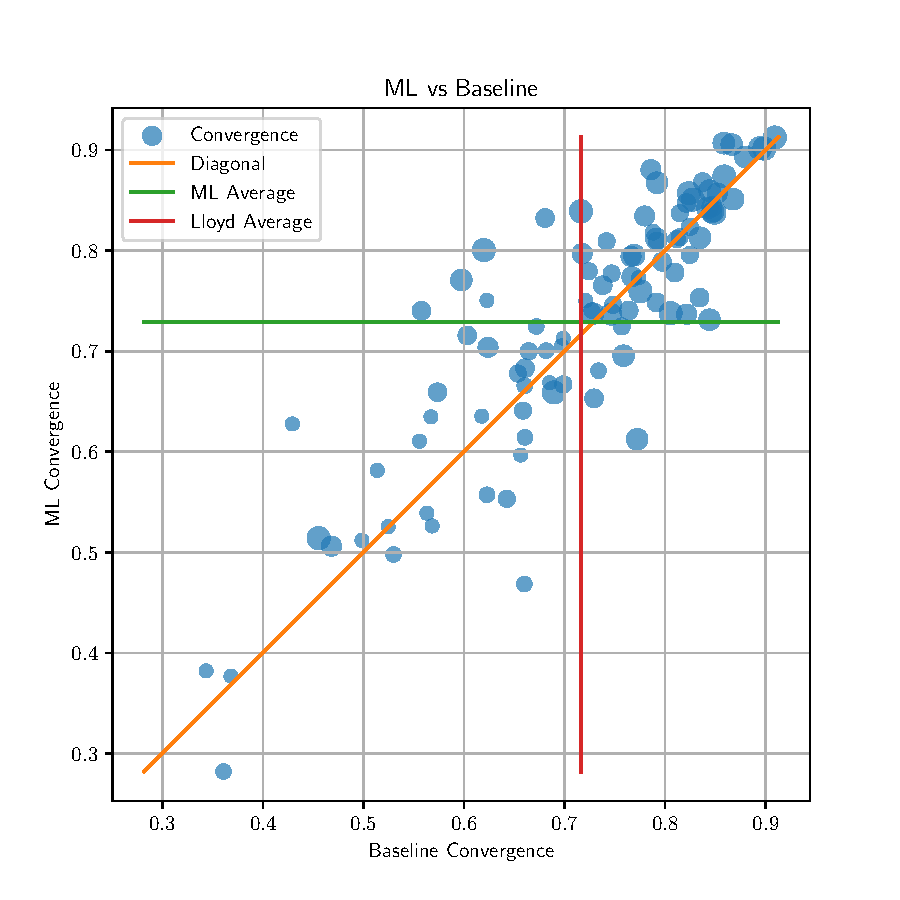
\includegraphics[width=\textwidth]{aniso3d_test_baseline_ml_convergence.pdf}
    \caption{Testing convergence}
  \end{subfigure}
  \caption{Convergence data for the ML AMG method vs a Lloyd and Jacobi SA method.  Values below the diagonal indicate a better convergence for the ML.  Markers are scaled by problem size.}
  \label{fig:aniso_conv}
\end{figure}
\bigskip\bigskip
\begin{figure}[!htb]
  \centering
  \begin{subfigure}[t]{0.49\textwidth}
    \centering
    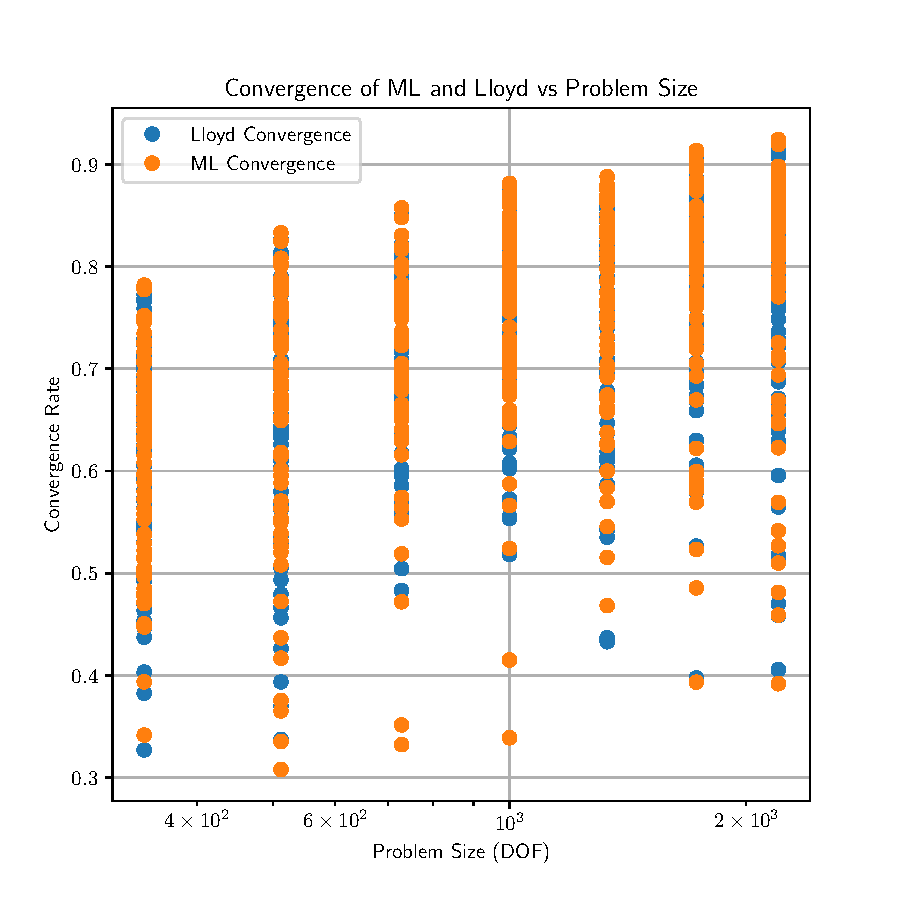
\includegraphics[width=\textwidth]{aniso3d_train_convergence_per_size.pdf}
    \caption{Training convergence}
  \end{subfigure}
  \begin{subfigure}[t]{0.49\textwidth}
    \centering
    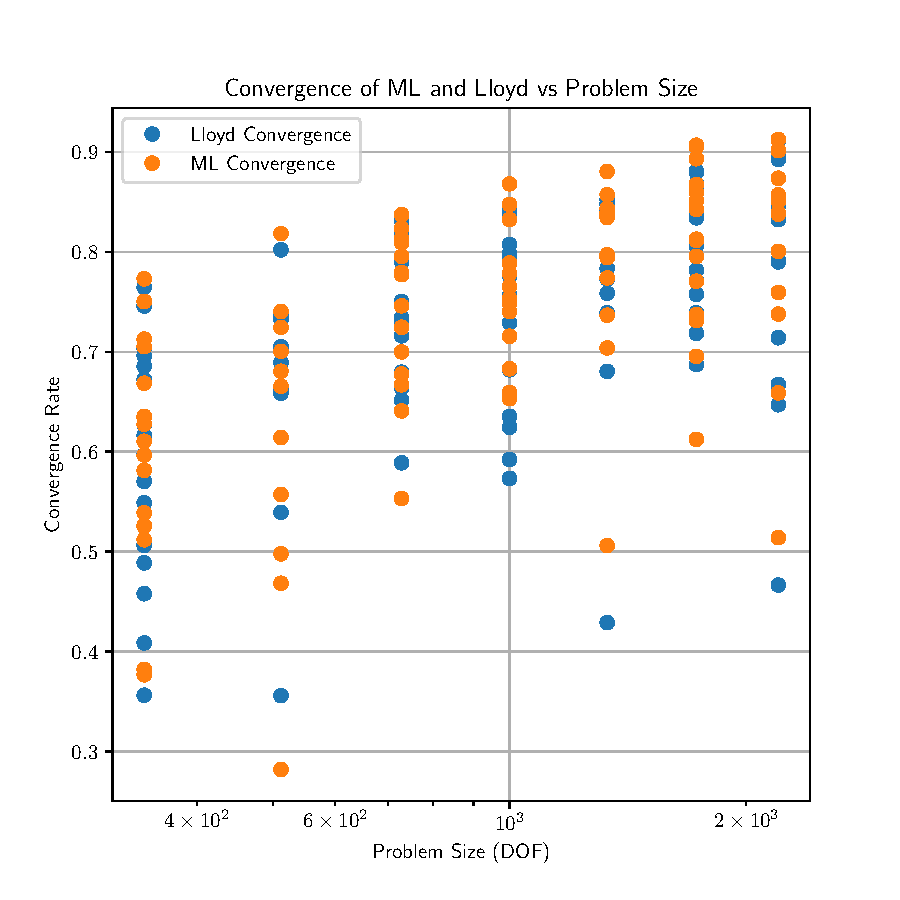
\includegraphics[width=\textwidth]{aniso3d_test_convergence_per_size.pdf}
    \caption{Testing convergence}
  \end{subfigure}
  \caption{Convergence data for the two methods plotted against problem size (DOF).}
  \label{fig:aniso_conv_per_size}
\end{figure}

\begin{figure}[h!]
  \centering
  \begin{subfigure}[t]{0.49\textwidth}
    \centering
    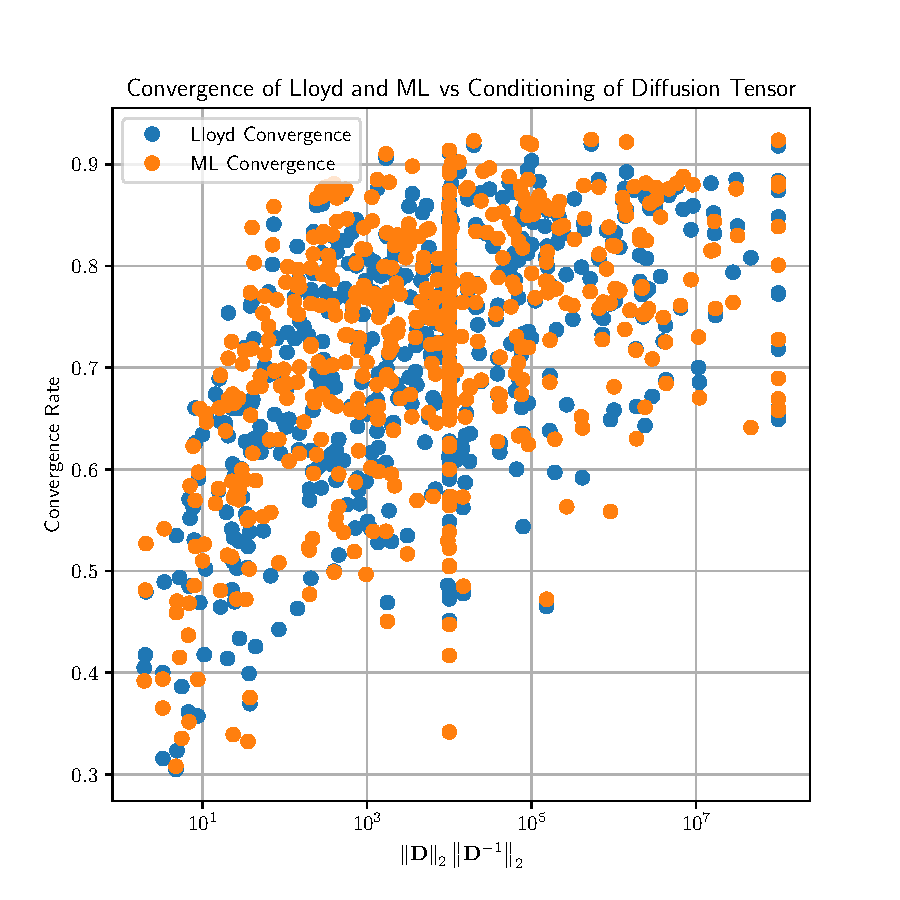
\includegraphics[width=\textwidth]{aniso3d_train_convergence_per_cond.pdf}
  \end{subfigure}
  \begin{subfigure}[t]{0.49\textwidth}
    \centering
    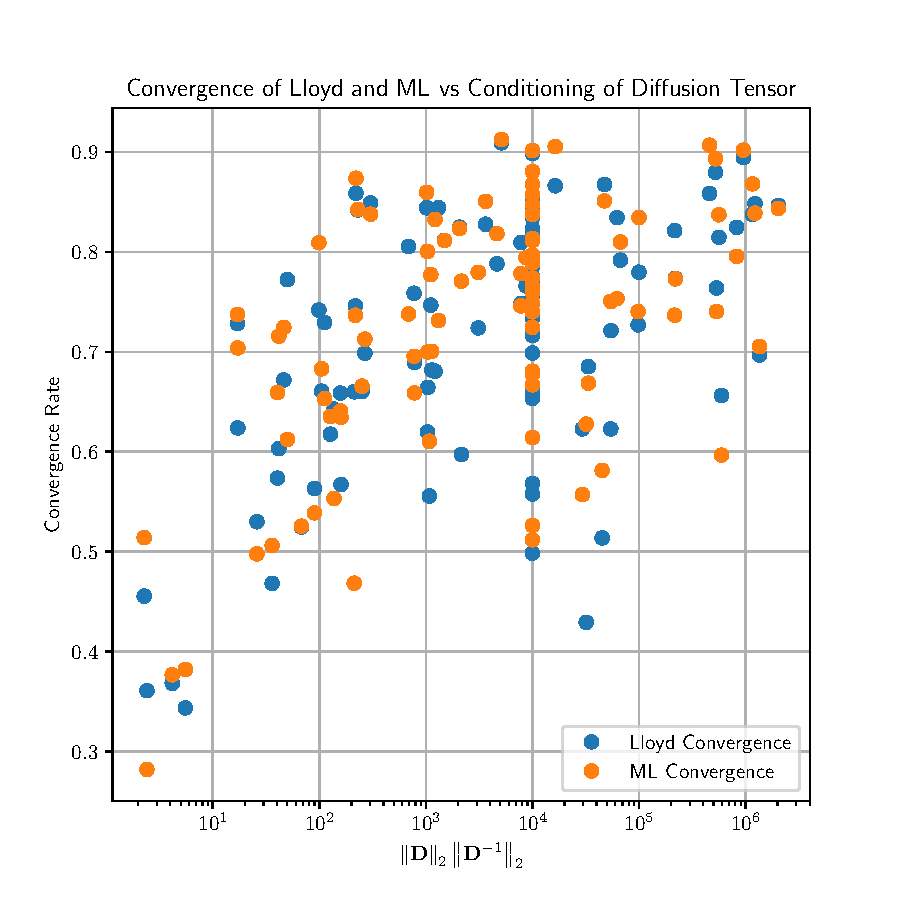
\includegraphics[width=\textwidth]{aniso3d_test_convergence_per_cond.pdf}
  \end{subfigure}
  \caption{Convergence on both datasets per ratio of extremal eigenvalues of the diffusion tensor.}
  \label{fig:aniso_conv_per_eps}
\end{figure}

\begin{figure}[h!]
  \centering
  \begin{subfigure}[t]{0.47\textwidth}
    \centering
    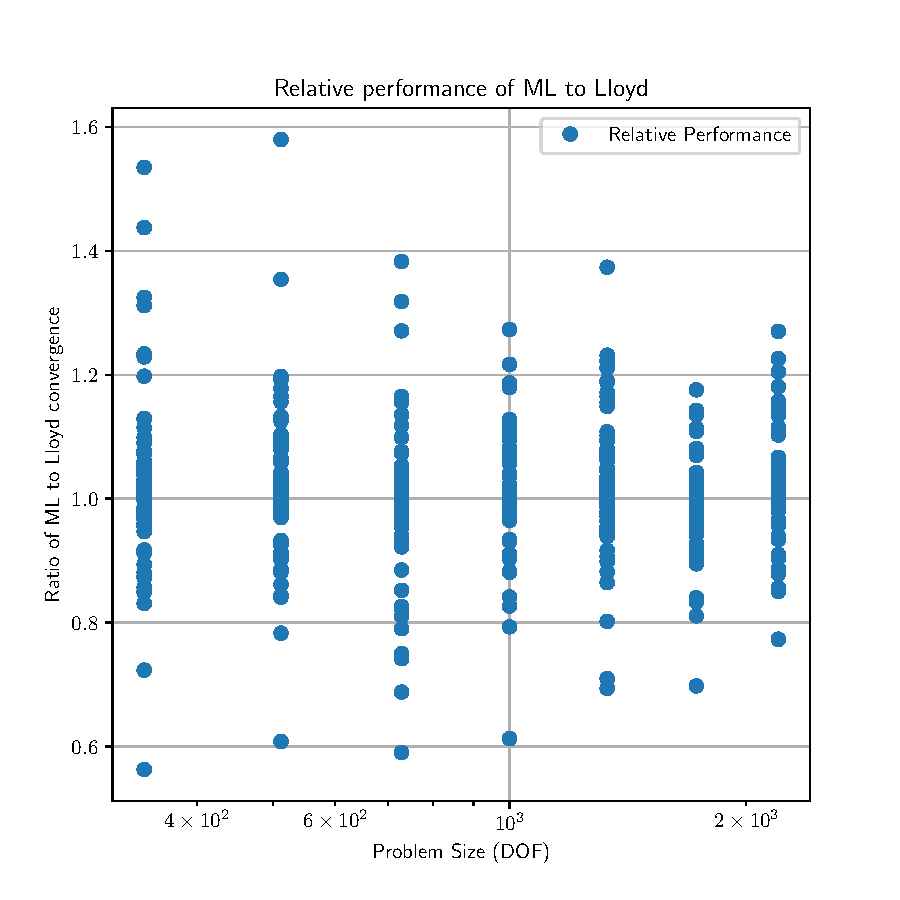
\includegraphics[width=\textwidth]{aniso3d_train_rel_perf.pdf}
    \caption{Relative training performance}
  \end{subfigure}
  \begin{subfigure}[t]{0.47\textwidth}
    \centering
    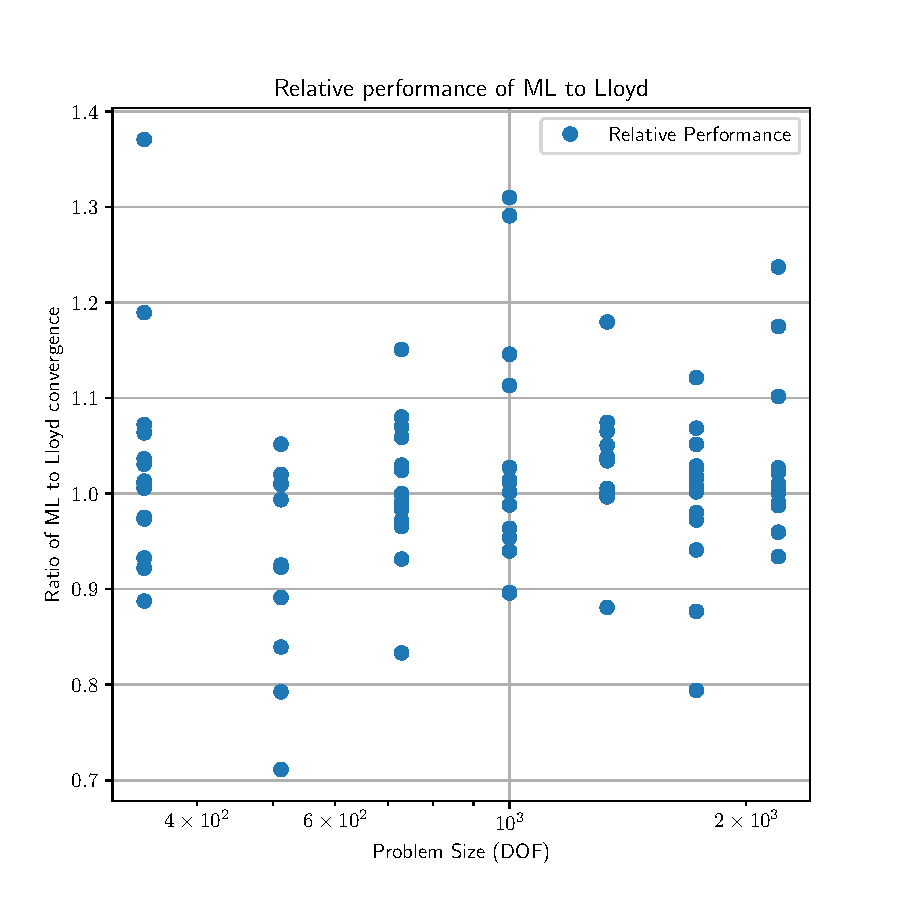
\includegraphics[width=\textwidth]{aniso3d_test_rel_perf.pdf}
    \caption{Relative testing performance}
  \end{subfigure}
  \caption{Relative performance of the ML to the Lloyd method, plotted against problem size.  Relative performance is obtained by dividing the ML convergence by the Lloyd convergence for each problem.  Values below $1$ indicate better ML performance, while values above $1$ indicate better baseline performance.}
  \label{fig:aniso_rel_conv}
\end{figure}

\bibliographystyle{siam}
\bibliography{navier}
\end{document}
